In this section, the External Components layer is described in detail. This layer is comprised of the physical parts that make the checkers game, this includes the checkers playing board, the checkers pieces, and the collection box.

\subsection{Layer Hardware}
N/A or The components of this layer do now require any computer system hardware but it deals with the hardware of the checkers game, including the playing board, the checkers pieces, and the collection box.

\subsection{Layer Operating System}
N/A

\subsection{Layer Software Dependencies}
N/A

%%%%%%%%%%%%%%%%%%%%%%%%%%%%%%%%%%%%%%%%%
\subsection{Playing Board}
The Playing Board is the physical wooden platform with distinct cells which the checkers game is played upon. 

\begin{figure}[h!]
	\centering
 	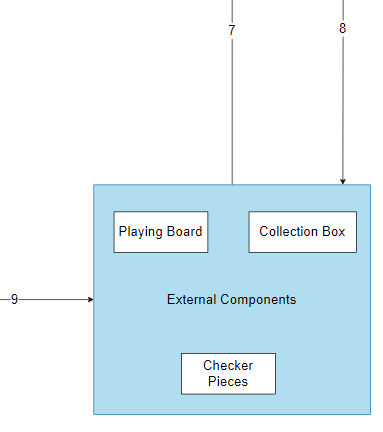
\includegraphics[width=0.60\textwidth]{images/externalComponents_subsystem.png}
 \caption{External components subsystem description diagram}
\end{figure}

\subsubsection{Subsystem Hardware}
% A description of any involved hardware components for the subsystem.
N/A

\subsubsection{Subsystem Operating System}
% A description of any operating systems required by the subsystem.
N/A

\subsubsection{Subsystem Software Dependencies}
% A description of any software dependencies (libraries, frameworks, design software for mechanical parts or circuits, etc) required by the subsystem.
N/A

\subsubsection{Subsystem Programming Languages}
% A description of any programming languages used by the subsystem.
N/A

\subsubsection{Subsystem Data Structures}
% A description of any classes or other data structures that are worth discussing for the subsystem. For example, data being transmitted from a microcontroller to a PC via USB should be first be assembled into packets. What is the structure of the packets?
N/A

\subsubsection{Subsystem Data Processing}
% A description of any algorithms or processing strategies that are worth discussing for the subsystem. If you are implementing a well-known algorithm, list it. If it is something unique to this project, discuss it in greater detail.
N/A

%%%%%%%%%%%%%%%%%%%%%%%%%%%%%%%%%%%%%%%%%
\subsection{Checkers Pieces}
The checkers pieces are the focus of the two players as they are the items that will be manipulated during the match. 

\subsubsection{Subsystem Hardware}
N/A

\subsubsection{Subsystem Operating System}
N/A

\subsubsection{Subsystem Software Dependencies}
% A description of any software dependencies (libraries, frameworks, design software for mechanical parts or circuits, etc) required by the subsystem.
N/A

\subsubsection{Subsystem Programming Languages}
% A description of any programming languages used by the subsystem.
N/A

\subsubsection{Subsystem Data Structures}
% A description of any classes or other data structures that are worth discussing for the subsystem. For example, data being transmitted from a microcontroller to a PC via USB should be first be assembled into packets. What is the structure of the packets?
N/A

\subsubsection{Subsystem Data Processing}
% A description of any algorithms or processing strategies that are worth discussing for the subsystem. If you are implementing a well-known algorithm, list it. If it is something unique to this project, discuss it in greater detail.
N/A

%%%%%%%%%%%%%%%%%%%%%%%%%%%%%%%%%%%%%%%%%
\subsection{Collection Box}
The collection box stands off to the side ready to hold the checkers pieces.

\subsubsection{Subsystem Hardware}
% A description of any involved hardware components for the subsystem.
N/A

\subsubsection{Subsystem Operating System}
% A description of any operating systems required by the subsystem.
N/A

\subsubsection{Subsystem Software Dependencies}
% A description of any software dependencies (libraries, frameworks, design software for mechanical parts or circuits, etc) required by the subsystem.
N/A

\subsubsection{Subsystem Programming Languages}
% A description of any programming languages used by the subsystem.
N/A

\subsubsection{Subsystem Data Structures}
% A description of any classes or other data structures that are worth discussing for the subsystem. For example, data being transmitted from a microcontroller to a PC via USB should be first be assembled into packets. What is the structure of the packets?
N/A

\subsubsection{Subsystem Data Processing}
% A description of any algorithms or processing strategies that are worth discussing for the subsystem. If you are implementing a well-known algorithm, list it. If it is something unique to this project, discuss it in greater detail.
N/A


